\documentclass[a4paper,10pt]{article}
\usepackage[T1]{fontenc}
\usepackage[utf8]{inputenc}
\usepackage{lmodern}
\usepackage{url,csquotes}
\usepackage{fancyhdr}
\usepackage{graphicx}
\usepackage{lastpage}
\usepackage{listings}
\usepackage{fancyref}
\usepackage{subfigure}

\usepackage{tabularx, booktabs ,multirow}
\usepackage{mathtools}

\usepackage{anysize} %%pour pouvoir mettre les marges qu'on veut 
\marginsize{2.5cm}{2.5cm}{2.5cm}{2.5cm} 

\usepackage{amsfonts,amssymb,amsmath,amsthm} 
\newcommand{\vect}[2]{ $\begin{pmatrix} #1 \\  #2 \end{pmatrix} $  }

\newcommand{\matrice}[3]{ \begin{pmatrix}  #1 &  #3 \\ #3  & #2 \end{pmatrix}   }

\newcommand{\norm}[1]{\left\lVert #1 \right\rVert} 
\newcommand{\norme}[1]{\left\lVert #1 \right\rVert_2} 
\newcommand{\fsurg}{\frac{f}{g}} 
\newcommand{\prodv}[2]{ #1^T #2 } 
\usepackage{enumerate} 

% Graph package
\usepackage{tikz}
\usetikzlibrary{arrows}

\newtheoremstyle{exostyle} 
{\topsep}% espace avant 
{\topsep}% espace apres 
{}% Police utilisee par le style de thm 
{}% Indentation (vide = aucune, \parindent = indentation paragraphe) 
{\bfseries}% Police du titre de thm 
{}% Signe de ponctuation apres le titre du thm 
{\newline}% Espace apres le titre du thm (\newline = linebreak) 
{\thmname{#1}\thmnote{ \normalfont{\textbf{#3}}}}% composants du titre du thm : \thmname = nom du thm, \thmnumber = numéro du thm, \thmnote = sous-titre du thm 

\theoremstyle{exostyle} 
\newtheorem{exercice}{Exercice} 
\newtheorem{rem}{Remark} 
\newtheorem{Sol}{Solution}
\newtheorem{theorem}{Theorem}
\begin{document}

\begin{center}
Master MVA \\
Probabilistic Graphical Models \\
DM 1 - 31/10/2016\\
Youssef Achari Berrada \\
\end{center}

\section{Learning in discrete graphical models}
In this example, we have a simple model with two nodes, represented by a plate: \\
\begin{center}
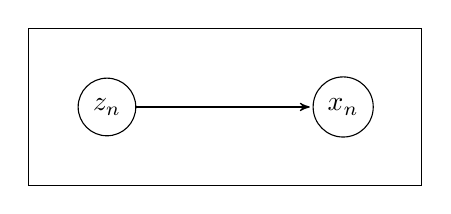
\begin{tikzpicture}[->,>=stealth',shorten >=1pt,auto,node distance=3cm,
                    thin,main node/.style={circle,draw}]
  \draw [thin] (-1,-1) rectangle (4,1);
%  \draw [thin] (2,-1) rectangle ;
  \node[main node] (1) {\textit{$z_n$}};
  \node[main node] (2) [right of=1] {\textit{$x_n$}};
  \path[every node/.style={font=\sffamily\small}]
  (1) edge node {} (2);
\end{tikzpicture}
\end{center}
$z$ and $x$ are discrete variables taking respectively $M$ and $K$ different values with $p(z_n = m) = \pi_m$ and $p(x_n=k | z_n=m) = \theta_{km}$. First, we observe that $ \sum_{m=1}^M \pi_m =1$ and $\sum_{k=1}^K \theta_{mk} = 1$ for each $m$.Then we have: 
\begin{align*}
p_{\theta,\pi}(z_n,x_n)  & = p_{\pi}(z_n) . p_{\theta}(x_n|z_n) \\
				&   = \prod_{m=1}^M \left( \pi_m^{z_n^m}  \prod_{k=1}^K \left( \theta_{mk}^{x_n^k}  \right)  \right) \\
\end{align*}
So the probability of the observation $x$: \\
\begin{align*}
p_{\theta,\pi}(z,x) &  = \prod_{n=1}^N \prod_{m=1}^M \left( \pi_m^{z_n^m}  \prod_{k=1}^K \left( \theta_{mk}^{x_n^k}  \right)  \right)  \\
					& = \prod_{m=1}^M  \left[ \prod_{n=1}^N ( \pi_m^{z_n^m} ) \prod_{k=1}^K \left( \prod_{n=1}^N ( \theta_{mk}^{x_n^k} )   \right) \right] \\
					& = \prod_{m=1}^M  \left[ \pi_m^{\sum_{n=1}^N z_n^m} \prod_{k=1}^K \left(\theta_{mk}^{\sum_{n=1}^N x_n^k}  \right) \right] 
\end{align*}
To calculate the maximum likelihood estimates, we take the logarithm of the last equation to obtain the $\log$ likelihood: \\
\begin{align*}
l_{\pi,\theta}(z,x)  & = \sum_{m=1}^M  \left[  \left(\sum_{n=1}^N z_n^m \right) \log(\pi_m)  +  \sum_{k=1}^K  \left(\sum_{n=1}^N x_n^k \right) \log(\theta_{mk}) \right] \\ 
					& = \sum_{m=1}^M  \left(\sum_{n=1}^N z_n^m \right) \log(\pi_m)  +  \sum_{m=1}^M  \sum_{k=1}^K  \left(\sum_{n=1}^N x_n^k \right) \log(\theta_{mk}) 
\end{align*}
The maximization over $(\pi,\theta)$ of the $\log$ likelyhood is a constrained optimization problem for which we use the Lagrange multipliers with $M+1$ constraints:  \\
\begin{align*}
\tilde{l}_{\pi,\theta}(z,x)  & = \sum_{m=1}^M  \left(\sum_{n=1}^N z_n^m \right) \log(\pi_m)  +  \sum_{m=1}^M  \sum_{k=1}^K  \left(\sum_{n=1}^N x_n^k \right) \log(\theta_{mk})   + \lambda (1 - \sum_{m=1}^M \pi_m ) + \sum_{m=1}^M  \gamma_m (1 - \sum_{k=1}^K \theta_{mk})
\end{align*}
The derivative over $\pi_m$: 
\begin{equation*}
\frac{\partial  \tilde{l}_{\pi,\theta}(z,x) }{\partial \pi_m} = \dfrac{\sum_{n=1}^N z_n^m }{\pi_m} - \lambda 
\end{equation*}
The derivative over $\theta_{mk}$:\\
\begin{equation*}
\frac{\partial  \tilde{l}_{\pi,\theta}(z,x) }{\partial \theta_{mk}} = \dfrac{\sum_{n=1}^N x_n^k }{\theta_{mk}} - \gamma_m
\end{equation*} 
By setting these partial derivatives equal to zero, we obtain: 
\begin{align*}
\sum_{n=1}^N z_n^m  = \lambda \pi_m & \underset{\text{After summing over m}}{\underbrace{\Longrightarrow}}    \lambda = N \\
\sum_{n=1}^N x_n^k  = \gamma_m \theta_{mk} & \underset{\text{After summing over k}}{\underbrace{\Longrightarrow}}    \gamma_m = N 
\end{align*} 
Finally, by substitution, we obtain: 
\begin{align*}
\hat{\pi}_{m,ML} & =  \frac{1}{N} \sum_{n=1}^N z_n^m \\
\hat{\theta}_{mk.ML} & = \frac{1}{N} \sum_{n=1}^N x_n^k 
\end{align*}
Noting that $ \sum_{n=1}^N z_n^m$ is the count of the number of times that the $m$th value is observed in $z$ and also $\sum_{n=1}^N x_n^k$ is the count of the number of times that the $k$th value is observed in $x$. We see that the maximum likelihood estimate is a sample proportion. 

\section{Linear classification}
\subsection{Generative model (LDA):}
\begin{enumerate}[(a)]
\item First, we know that $y \sim \textit{Bernoulli}(\pi)$ and $ x | y=i \sim \textit{Normal}(\mu_i,\Sigma)$. So we can express: 
\begin{align*}
p(y=1) = \pi  \quad ,\quad p(y=0) = 1- \pi \quad ,\quad  p_{\mu_i,\Sigma}(X=x|y=i)  = \frac{1}{\sqrt{(2\pi)^2 |\Sigma|}} \exp\left(-\frac{1}{2} (x-\mu_i)^T \Sigma^{-1} (x-\mu_i) \right)
\end{align*}
For $i \in \{0,1\}$, and if $X_1, ..., X_N \sim  \textit{Normal}(\mu_i,\Sigma) $,iid., we have seen in the lecture 2 that: 
\begin{align*}
\hat{\mu}_i & = \frac{1}{N} \sum_{k=1}^N x_k \\
\hat{\Sigma}_i & = \frac{1}{N}	\sum_{k=1}^N (x_k - \hat{\mu}_i)^T	(x_k - \hat{\mu}_i)
\end{align*}
In the experiment, the fisher assumption is considered by taken $\hat{\Sigma} = \dfrac{\hat{\Sigma}_1 + \hat{\Sigma}_0}{2}$.

\item 


\begin{align*}
p(y=1|X=x) & = \dfrac{p(X=x|y=1) p(y=1)}{p(X=x|y=1) p(y=1) + p(X=x|y=0) p(y=0)} \\
				& = \dfrac{\pi \exp\left(-\frac{1}{2} (x-\mu_1)^T \Sigma^{-1} (x-\mu_1) \right)}{ \pi \exp\left(-\frac{1}{2} (x-\mu_1)^T \Sigma^{-1} (x-\mu_1)\right) + (1-\pi) \exp\left(-\frac{1}{2} (x-\mu_0)^T \Sigma^{-1} (x-\mu_0)\right)} \\
				& = \dfrac{1}{ 1 + \frac{1-\pi}{\pi} \exp\left( - \frac{1}{2} [  (x-\mu_0)^T \Sigma^{-1} (x-\mu_0)-(x-\mu_1)^T \Sigma^{-1} (x-\mu_1) ] \right)} \\
\end{align*}
We can proove that: 
\begin{align*}
(x-\mu_0)^T \Sigma^{-1} (x-\mu_0)-(x-\mu_1)^T \Sigma^{-1} (x-\mu_1) & = 2 (x - \frac{\mu_0 + \mu_1}{2})^T \Sigma^{-1} (\mu_1 - \mu_0)
\end{align*}
Then we conclude that:
\begin{align*}
p(y=1|X=x) & = \dfrac{1}{ 1 + \frac{1-\pi}{\pi} \exp\left( - (x - \frac{\mu_0 + \mu_1}{2})^T \Sigma^{-1} (\mu_1 - \mu_0) \right)}
\end{align*}
\item So we conclude that: 
\begin{align*}
p(y=1|X=x) > 0.5 & \Leftrightarrow (x - \frac{\mu_0 + \mu_1}{2})^T \Sigma^{-1} (\mu_1 - \mu_0) > \log(\frac{1-\pi}{\pi})
\end{align*}
which define a halfspace that depend on the value of $\pi$. 
\begin{figure}[!h]
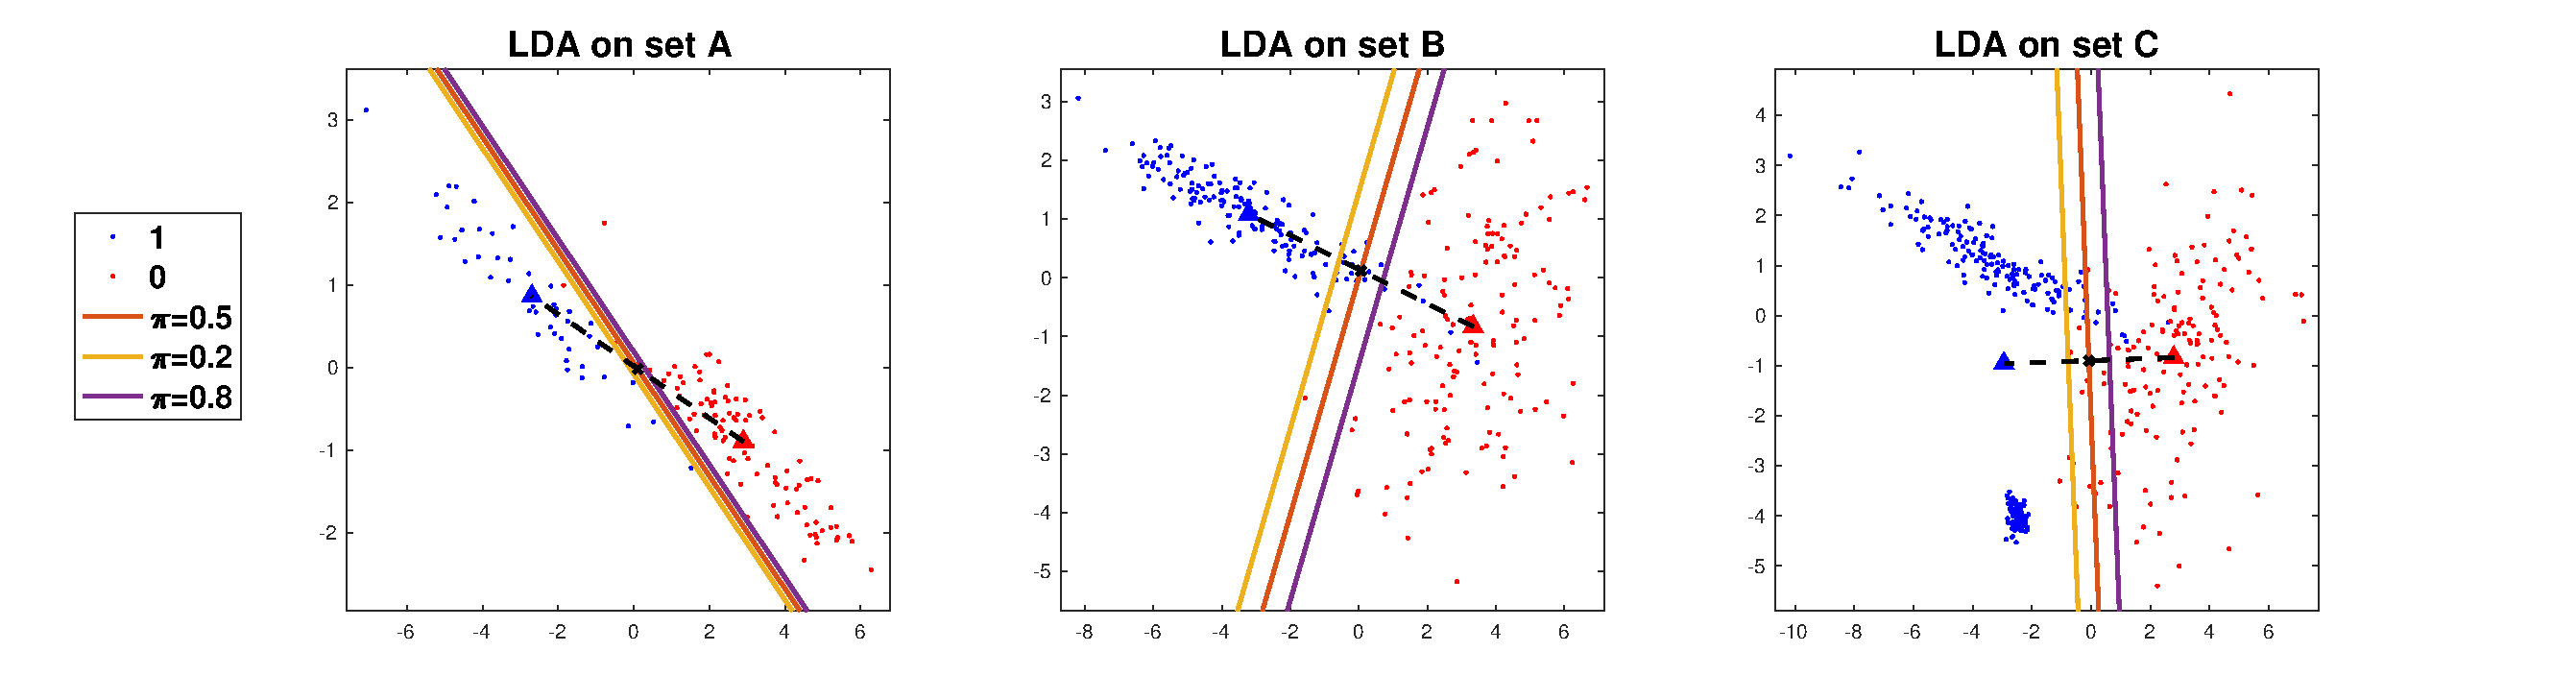
\includegraphics[width=\textwidth]{classification_data_HWK1/classification_data_HWK1/LDATrain.eps} 
\caption{LDA on the train data with different value of $\pi$.}
\end{figure}

\begin{table}[!h]
\centering
\caption{Learnt parameters for LDA}

\begin{tabular}{l | c|c|c}
      & A & B & C \\ \hline \hline
$\mu_0  $ &  \vect{ 2.8997}{-0.8939}   &   \vect{3.3407}{-0.8355}  &  \vect{2.7930}{-0.8384}   \\ \hline
\hline
$\mu_1  $   & \vect{-2.6923}{0.8660}  &   \vect{-3.2167}{1.0831}  &  \vect{-2.9423}{-0.9578}   \\ \hline
\hline
$\Sigma  $ & $  \matrice{2.5468}{0.6427}{-1.1927}  $ & $  \matrice{3.3687}{1.7497}{-0.1361}  $  & $  \matrice{2.8996}{4.7676}{-0.2574}  $ 
\end{tabular}
\end{table}

\end{enumerate}

\subsection{Logistic Regression:} 
\begin{enumerate}[(a)]
\item $f(x) = w^T x + b$ with the parameters $ w \in \mathbb{R}^2$ and $b \in \mathbb{R}$. In order to include the constant term, one can do the following transformation on $f$ : 
\begin{align*}
f(x) = \begin{pmatrix} b \\ w \end{pmatrix}^T   \begin{pmatrix} 1 \\ x \end{pmatrix}
\end{align*}
and then consider $\tilde{w} = \begin{pmatrix} b \\ w \end{pmatrix} \in  \mathbb{R}^3$. \\
After learning the parameters $w$ and $b$ using the \textit{Iterative Reweighted Linear Square} method. 

\begin{table}[!h]
\centering
\caption{Learnt parameters by logistic regression.}
\begin{tabular}{|c|c|c|c|l}
\cline{1-4}
Logistic Regression & Train A & Train B & Train C &  \\ \cline{1-4}
$w_1 $            &   $-989.0780$    &       $-6.4128 $    &    $-7.1788$     &  \\ \cline{1-4}
$w_2$                &    $-637.7548 $     &    $ 1.6720$     &   $1.6198$      &  \\ \cline{1-4}
$ b $                &    $-215.6995$     &     $1.3706$    &   $2.0556$      &  \\ \cline{1-4}
\end{tabular}
\end{table}
\item 
\begin{align*}
p(y=1|x) = 0.5 &  \Leftrightarrow \begin{pmatrix} b \\ w \end{pmatrix}^T  \begin{pmatrix} 1 \\ x \end{pmatrix} = 0\\
				& \Leftrightarrow w^T x + b = 0 
\end{align*} 
which define a line in $\mathbb{R}^2$. 
\begin{figure}[!h]
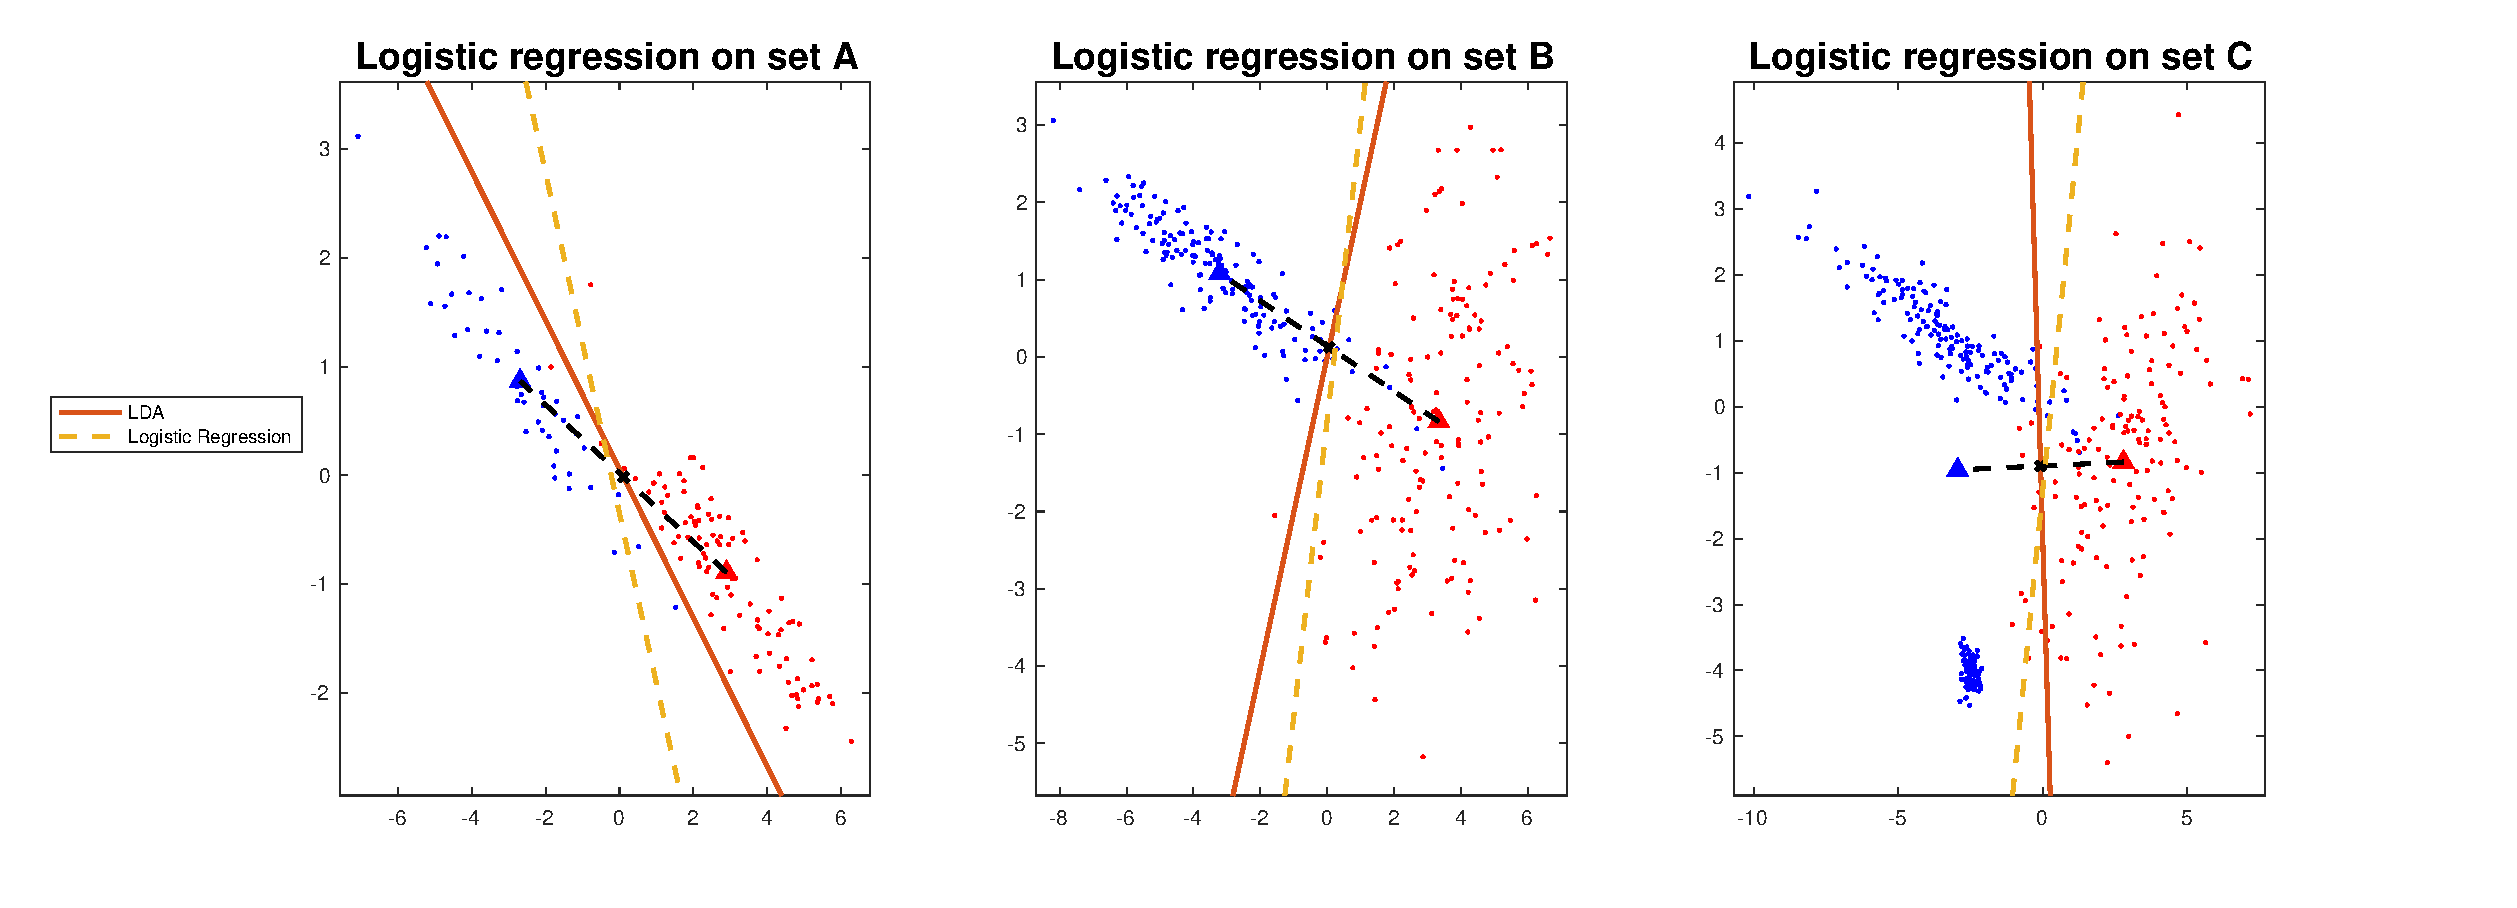
\includegraphics[width=\textwidth]{classification_data_HWK1/classification_data_HWK1/logR.eps} 
\caption{Logistic regression on the training data versus LDA.}
\end{figure}
\end{enumerate}

\subsection{Linear Regression:}


\begin{table}[!h]
\centering
\caption{Learnt parameters by linear regression.}
\begin{tabular}{|c|c|c|c|l}
\cline{1-4}
Linear Regression & Train A & Train B & Train C &  \\ \cline{1-4}
$w_1 $            &   $-0.8118$    &       $-0.3920 $    &    $-0.4161$     &  \\ \cline{1-4}
$w_2$                &    $-0.4266 $     &    $ 0.0846$     &   $-0.0388$      &  \\ \cline{1-4}
$ b $                &    $0.3333$     &     $0.5000$    &   $0.6250$      &  \\ \cline{1-4}
\end{tabular}
\end{table}



\begin{figure}[!h]
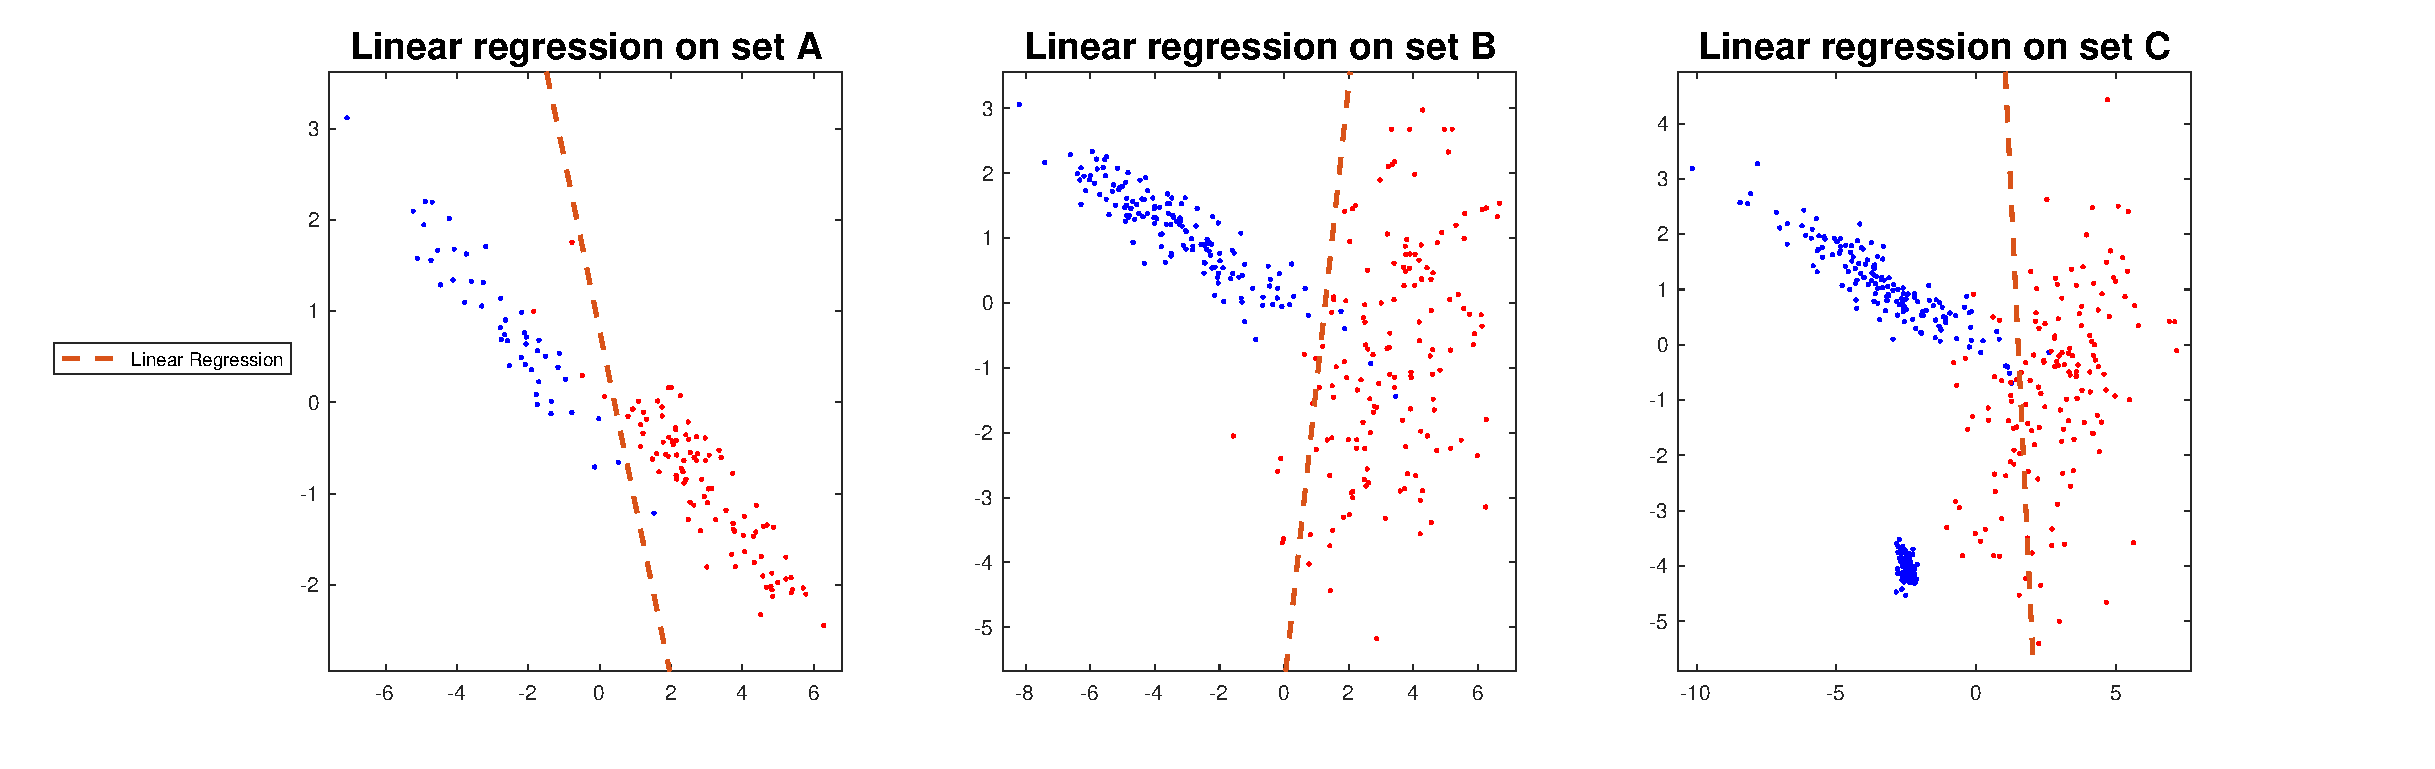
\includegraphics[width=\textwidth]{classification_data_HWK1/classification_data_HWK1/LinR.eps} 
\caption{Linear regression on the training data.}
\end{figure}

\newpage
\subsection{Testing:}

\begin{table}[!h]
\centering
\caption{Misclassification Error}
\begin{tabular}{llccc}
\multicolumn{2}{l}{}   & A & B & C \\
\multirow{2}{*}{\textbf{LDA}}                 & Train & $\textbf{0.0133}$   & $0.0300 $  &  $0.0500$ \\
                                      			& Test  & $0.0240$  & $\textbf{0.0415}$  & $0.0387$   \\
\multirow{2}{*}{\textbf{Logisctic Regression}} & Train & $0.0333$   &  $\textbf{0.0267}$ &  $\textbf{0.0400}$ \\
                                      & Test  & $\textbf{0.0180}$  &  $0.0440$ & $\textbf{0.0257}$  \\
\multirow{2}{*}{Linear Regression}    & Test  &  $0.0400$ & $0.0400$  & $0.0975$   \\
                                      & Train &  $0.0360$ & $0.0670$  &  $0.0780$
\end{tabular}
\end{table}
As we see in the table above, the logistic model is the best one, in particular on the set C where the model performs far better than the other two models. \\
The LDA perform well on the set A because indeed, the fisher assumption is verified on that particular set. \\ 
The LDA and Logistic model yield to very similar results on the set B. The Linear model performs bad on the models where there is outliers like on the set C, because it does not take into account the distribution of the data. \\

\begin{figure}[!h]
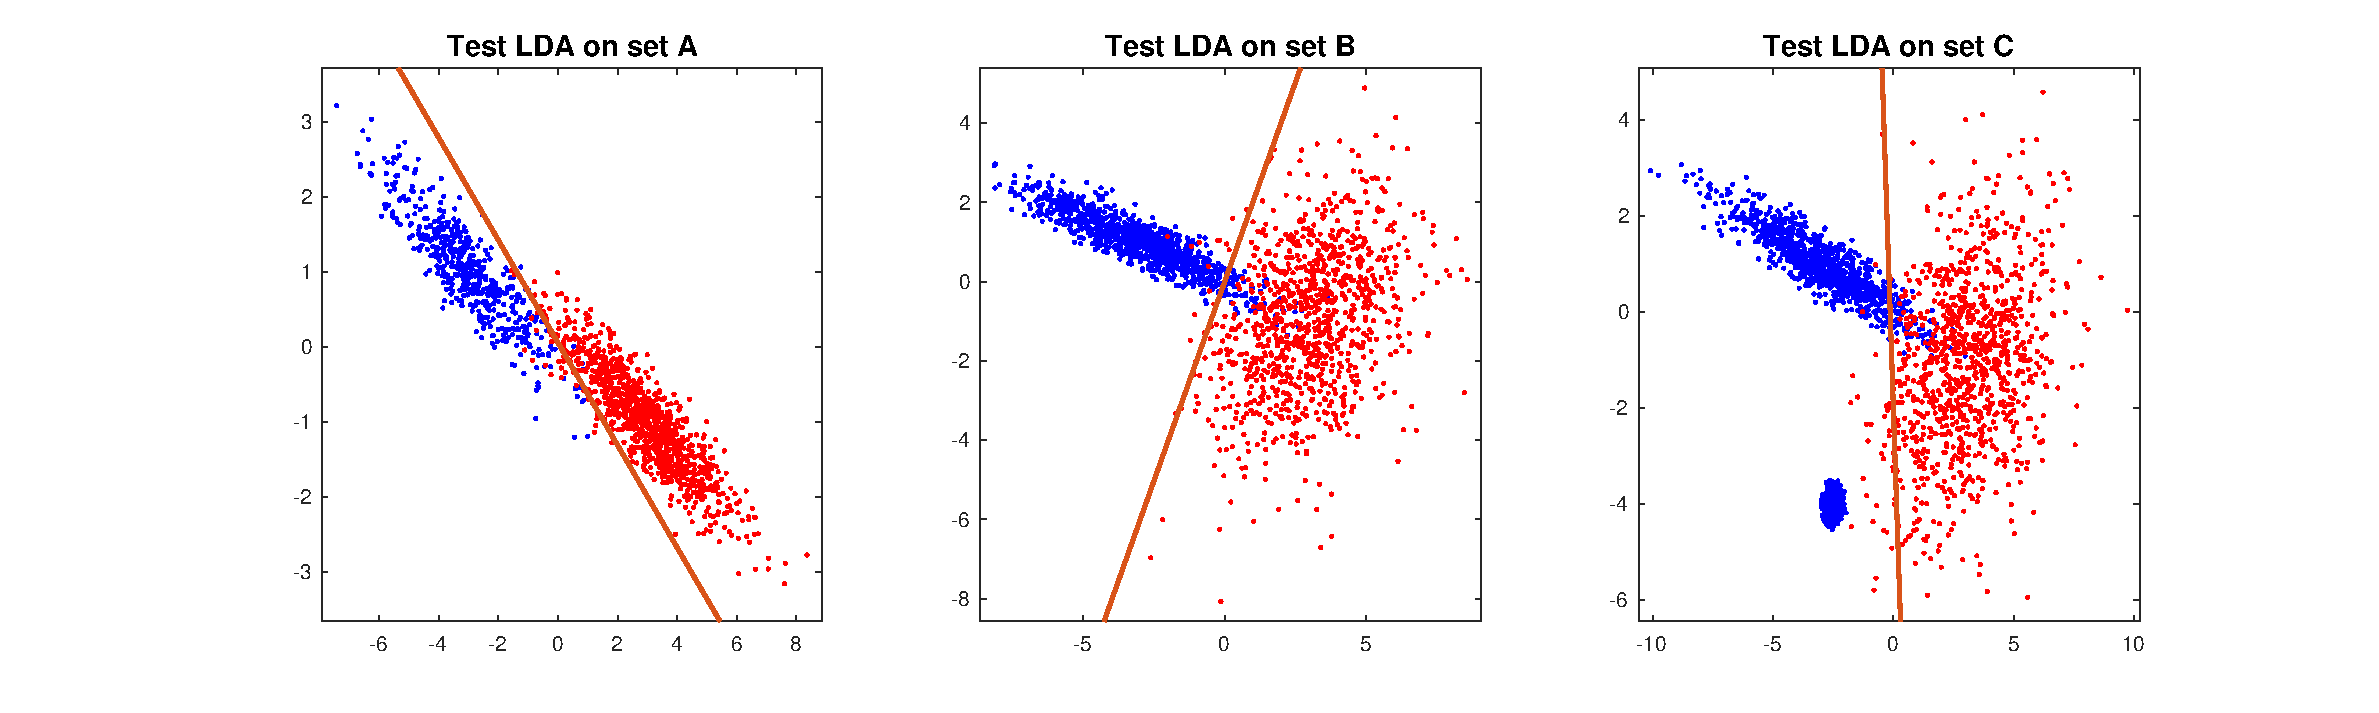
\includegraphics[width=\textwidth]{classification_data_HWK1/classification_data_HWK1/ldaTest.eps} 
\caption{Testing LDA.}
\end{figure}

\begin{figure}[!h]
\includegraphics[width=\textwidth]{classification_data_HWK1/classification_data_HWK1/logTest.eps} 
\caption{Testing logistic regression.}
\end{figure}

\begin{figure}[!h]
\includegraphics[width=\textwidth]{classification_data_HWK1/classification_data_HWK1/linTest.eps} 
\caption{Testing linear regression.}
\end{figure}

\newpage
\subsection{QDA model:}
\begin{enumerate}[(a)]
\item The parameters $\mu_0$ and $\mu_1$ are the same as in the LDA model. See table 1. 
\begin{table}[!h]
\centering
\caption{Learnt parameters for QDA}

\begin{tabular}{l | c|c|c}
      & A & B & C \\ \hline \hline
$\Sigma_0  $ & $  \matrice{2.5468}{0.6427}{-1.1927}  $ & $  \matrice{3.3687}{1.7497}{-0.1361}  $  & $  \matrice{2.8996}{4.7676}{-0.2574}  $\\ \hline
\hline
$\Sigma_1 $ & $  \matrice{2.5468}{0.6427}{-1.1927}  $ & $  \matrice{3.3687}{1.7497}{-0.1361}  $  & $  \matrice{2.8996}{4.7676}{-0.2574}  $ 
\end{tabular}
\end{table}

\item
\begin{align*}
p(y=1|X=x) & = \dfrac{p(X=x|y=1) p(y=1)}{p(X=x|y=1) p(y=1) + p(X=x|y=0) p(y=0)} \\
				& = \dfrac{\pi \exp\left(-\frac{1}{2} (x-\mu_1)^T \Sigma^{-1}_1 (x-\mu_1) \right)}{ \pi \exp\left(-\frac{1}{2} (x-\mu_1)^T \Sigma^{-1}_1 (x-\mu_1)\right) + (1-\pi) \exp\left(-\frac{1}{2} (x-\mu_0)^T \Sigma^{-1}_0 (x-\mu_0)\right)} \\
				& = \dfrac{1}{ 1 + \frac{1-\pi}{\pi} \exp\left( - \frac{1}{2} [  (x-\mu_0)^T \Sigma^{-1}_0 (x-\mu_0)-(x-\mu_1)^T \Sigma^{-1}_1 (x-\mu_1) ] \right)} \\
\end{align*}
\begin{align*}
p(y=1|X=x) = 0.5 & \Leftrightarrow   (x-\mu_0)^T \Sigma^{-1}_0 (x-\mu_0)-(x-\mu_1)^T \Sigma^{-1}_1 (x-\mu_1)  = 2  \log(\frac{1-\pi}{\pi})
\end{align*}
which define a conic.
\begin{figure}[!h]
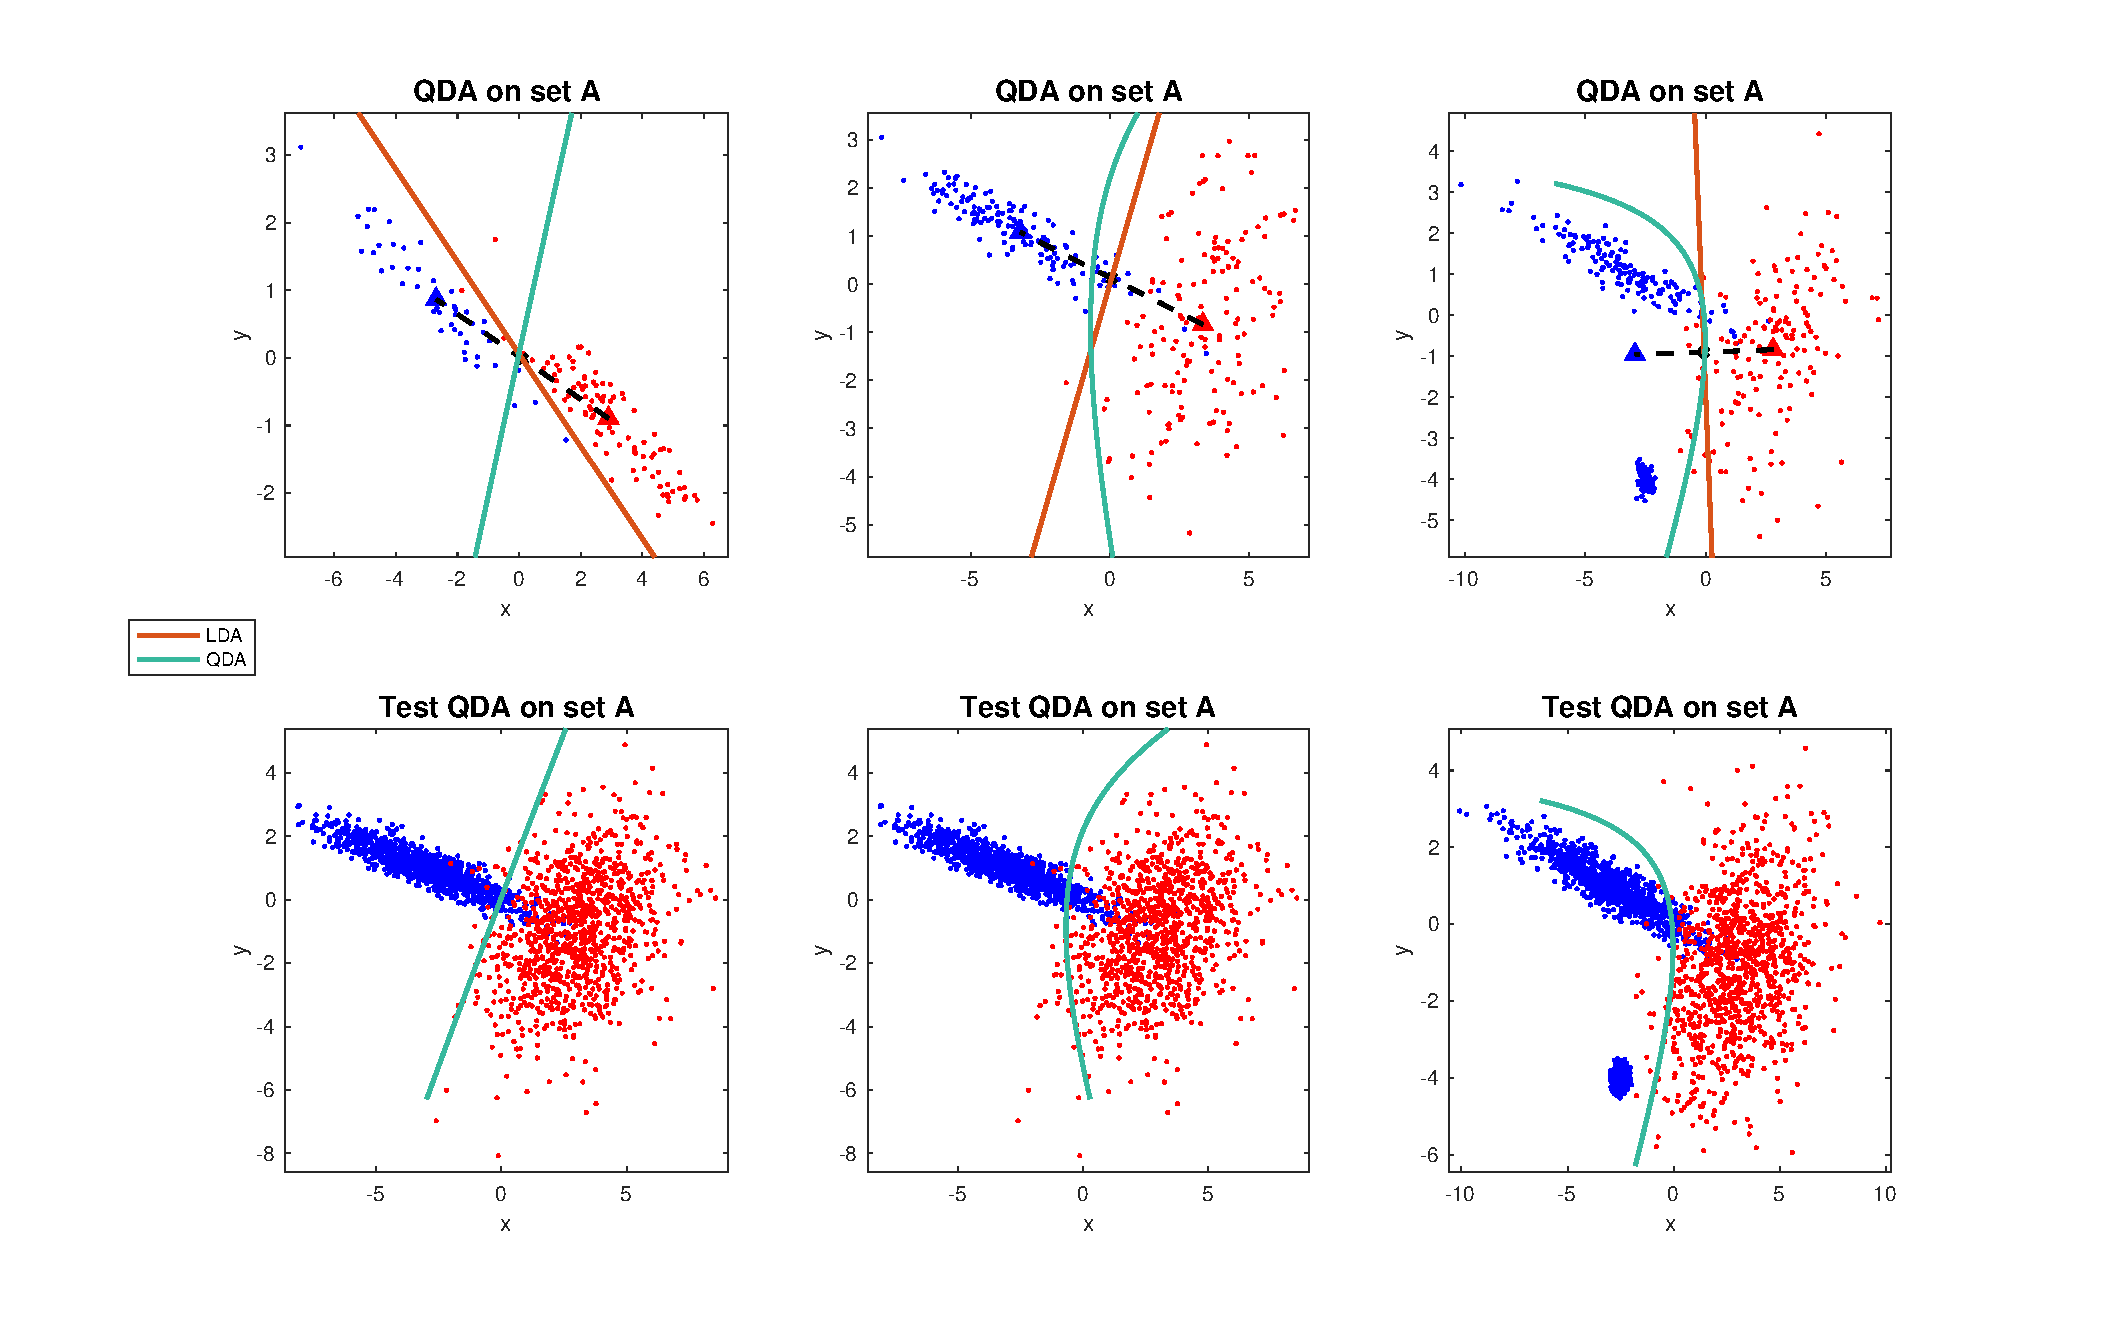
\includegraphics[width=\textwidth]{classification_data_HWK1/classification_data_HWK1/QDA.eps} 
\caption{QDA vs LDA.}
\end{figure}
\item Here is the misclassification error on the QDA training and test sets. 
\begin{table}[!h]
\centering
\caption{QDA Misclassification Error}
\begin{tabular}{clccc}
\multicolumn{2}{l}{}         & A & B & C \\
\multirow{2}{*}{QDA} & Train & $0.0133$  & $0.0233$  &  $0.0525$ \\
                     & Test  &  $0.0213$ &  $0.0235$ &  $0.0370$
\end{tabular}
\end{table}

\item If we compare the misclassification errors between the QDA and LDA models, they are very similar on set A, because the QDA and the LDA are equivalent on set A as $\Sigma_1 \sim \Sigma_2$.\\
The QDA model is better than the LDA model for the set B, because the QDA model now take into account the non similarity between $\Sigma_1$ and $\Sigma_2$. We can notice a high improvement on the test set B by the QDA model indeed. \\ 
We could notice that the QDA classification has less error that the LDA classification on the training set C and in opposite the QDA classification performs lower than the LDA one on the test set C. This is basically what happens when we have overfitting. And it is normal because the QDA model involve quadratic terms on $x$ and $y$ but the LDA involve only linear terms on $x$ and $y$. But in this experiment, the QDA model is better that the LDA one on both the training and the test set C.  

\end{enumerate}

\end{document}
